%!TEX program = lualatex
% Unofficial University of Cambridge Poster Template
% https://github.com/andiac/gemini-cam
% a fork of https://github.com/anishathalye/gemini
% also refer to https://github.com/k4rtik/uchicago-poster

\documentclass[final]{beamer}

% ====================
% Packages
% ====================

\usepackage[T1]{fontenc}
\usepackage{lmodern}
\usepackage[orientation=portrait,size=a0,scale=1.06]{beamerposter}
\usetheme{gemini}
\usecolortheme{nott}
\usepackage{graphicx}
\usepackage{booktabs}
\usepackage[numbers]{natbib} % o [authoryear] según prefieras
\usepackage{tikz}
\usepackage{pgfplots}
\pgfplotsset{compat=1.14}
\usepackage{anyfontsize}

\providecommand{\abs}[1]{\left|#1\right|}
\providecommand{\norm}[1]{\left\|#1\right\|}


% ====================
% Lengths
% ====================

% If you have N columns, choose \sepwidth and \colwidth such that
% (N+1)*\sepwidth + N*\colwidth = \paperwidth
\newlength{\sepwidth}
\newlength{\colwidth}
\setlength{\sepwidth}{0.025\paperwidth}
\setlength{\colwidth}{0.45\paperwidth}

\newcommand{\separatorcolumn}{\begin{column}{\sepwidth}\end{column}}

% ====================
% Title
% ====================

\title{Models of the universe from differential geometry.}

\author{Andrés David Cadena Simons}

\institute[shortinst]{Departamento de Matemáticas, Universidad Nacional de Colombia sede Bogotá.}

% ====================
% Footer (optional)
% ====================

\footercontent{
  Geometría Diferencial --- 2025 \hfill
  \href{mailto:acadenas@unal.edu.co}{acadenas@unal.edu.co}}
% (can be left out to remove footer)


% ====================
% Logo (optional)
% ====================

% use this to include logos on the left and/or right side of the header:
\logoright{\hspace{-20ex}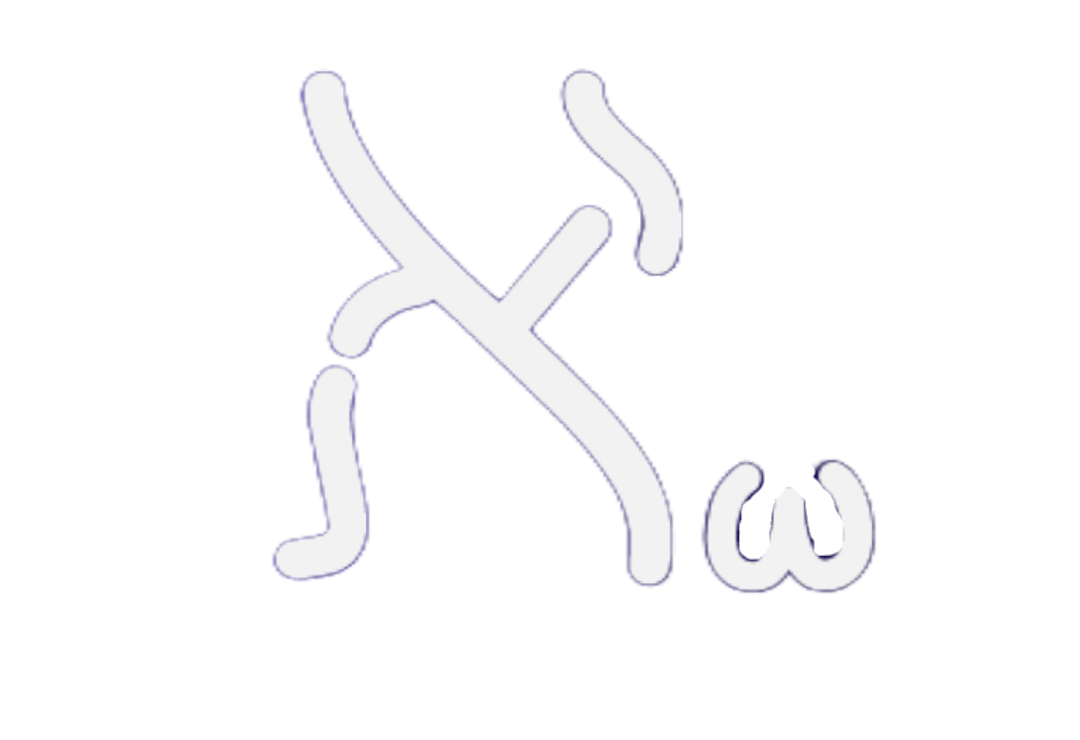
\includegraphics[height=6cm]{logos/alepth.png}}
\logoleft{\hspace{20ex}
\includegraphics[height=6cm]{logos/logo.png}}

% ====================
% Body
% ====================

\begin{document}

% Refer to https://github.com/k4rtik/uchicago-poster
% logo: https://www.cam.ac.uk/brand-resources/about-the-logo/logo-downloads
% \addtobeamertemplate{headline}{}
% {
%     \begin{tikzpicture}[remember picture,overlay]
%       \node [anchor=north west, inner sep=3cm] at ([xshift=-2.5cm,yshift=1.75cm]current page.north west)
%       {\includegraphics[height=7cm]{logos/unott-logo.eps}}; 
%     \end{tikzpicture}
% }

\begin{frame}[t]
\begin{columns}[t]
\separatorcolumn

\begin{column}{\colwidth}

  \begin{block}{Abstract}
    The document provides a clear and accessible introduction to the idea that gravity is a manifestation of spacetime curvature, as proposed by Einstein in his theory of general relativity.
    \begin{enumerate}
      \item Geodesics and curvature: It explains that the natural path of objects in curved spacetime is a geodesic, which generalizes the concept of a straight line.
      \item Gravity as geometry: Instead of viewing gravity as an instantaneous force (as in Newtonian theory), Einstein proposed that objects follow the curvature of spacetime shaped by the presence of matter.
      \item Models of the universe: Three types of universe are presented depending on their curvature:
      \begin{enumerate}[(a)]
        \item Flat (zero curvature).
        \item Spherical (positive curvature, closed universe).
        \item Hyperbolic (negative curvature, open universe).\\
          The sum of the angles in a triangle varies with the type of curvature.
      \end{enumerate}
      \item Escape velocity and black holes: The concept of escape velocity is introduced as the minimum needed to break free from a gravitational field. If this velocity equals the speed of light, a black hole forms. The Schwarzschild radius is derived from this idea, showing its dependence on the object's mass.
    \end{enumerate}
    \begin{center}
      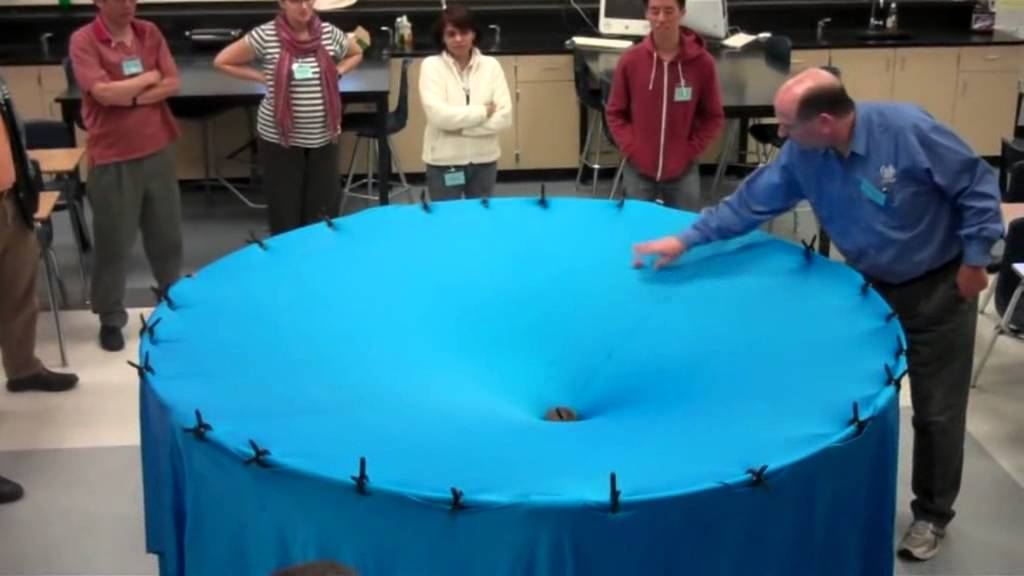
\includegraphics[scale=0.5]{manta.jpg}
    \end{center}
  \end{block}

  \begin{block}{Introduction}
  Since ancient times, humans have questioned the nature of the universe. For centuries, Newton's gravity explained the motion of celestial bodies as an attractive force. But Einstein redefined gravity as the curvature of spacetime caused by matter and energy.\\
  This insight explained phenomena like black holes and cosmic expansion, showing that objects follow curved paths —geodesics— through a deformed spacetime. Understanding the universe requires studying its curvature and concepts like escape velocity.
  \begin{center}
    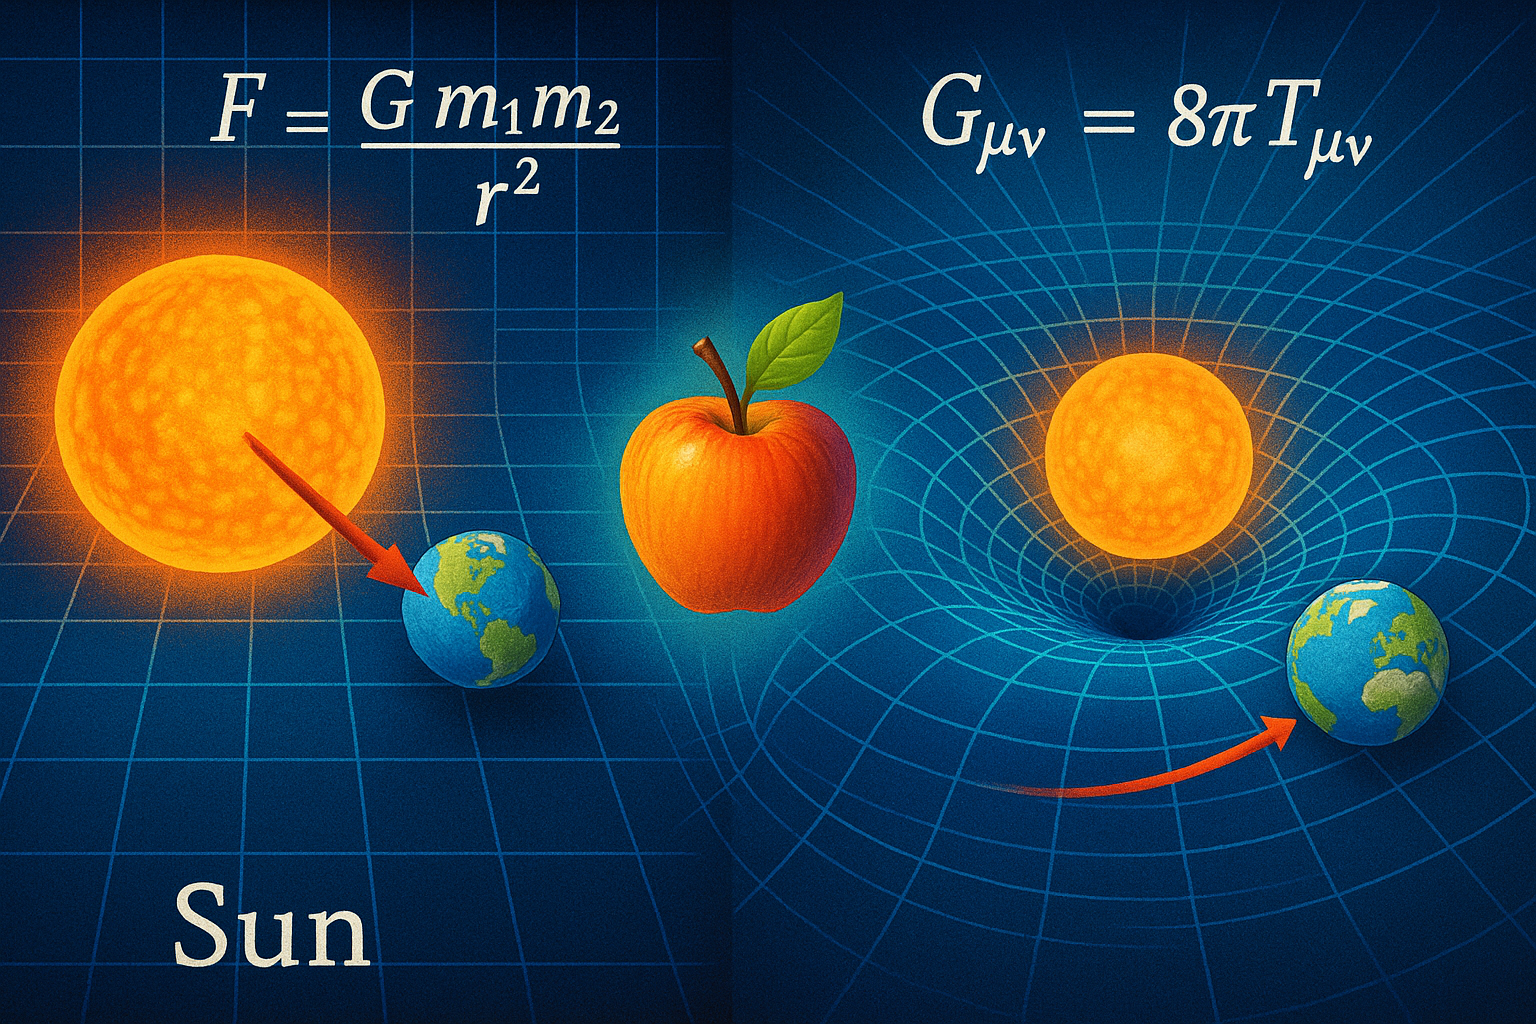
\includegraphics[scale=0.3]{chatgptimagen2.png}  
  \end{center}
  
  \end{block}

  \begin{alertblock}{Models of the Universe from the Perspective of Differential Geometry}
    Since general relativity, the geometric structure of the universe has become essential to understanding its behavior. Spacetime is modeled as a four-dimensional Lorentzian manifold, where curvature—determined by mass and energy—governs the motion of matter and light.

    \textbf{\large Curvature and Global Structure}

      \textit{Curvature} is a tool that characterizes the local geometry of a manifold. There are several notions of curvature (sectional, scalar, Ricci), but in cosmology, the case of manifolds with \textit{constant curvature} is especially relevant. Each of these geometries gives rise to a different model of the universe: 
        \begin{itemize}
          \item \textbf{Closed universe:} positive curvature (e.g., 3-sphere), triangle angle sum $> 180^\circ$.
          \item \textbf{Flat universe:} zero curvature ($\mathbb{R}^3$), triangle angle sum = $180^\circ$.
          \item \textbf{Open universe:} negative curvature (hyperboloid), triangle angle sum $< 180^\circ$.
        \end{itemize}
        This classification is formalized in the FLRW metric:
        \begin{align*}
        ds^2 = -c^2 dt^2 + a(t)^2 \left( \frac{dr^2}{1 - kr^2} + r^2 d\Omega^2 \right),
        \end{align*}
        where $k \in \{-1, 0, 1\}$ represents spatial curvature.
        \begin{center}
          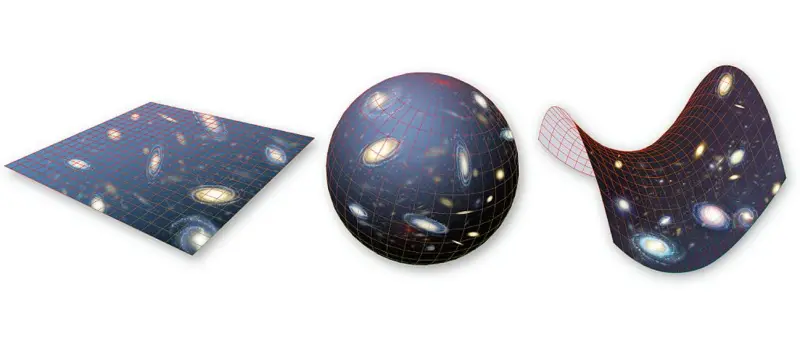
\includegraphics[scale=0.8]{curvaturuniverso.jpg}
        \end{center}        
        \textbf{\large Light, Curvature, and Black Holes}

        In relativity, light follows null geodesics, satisfying
        \begin{align*}
        g(\dot{\gamma}, \dot{\gamma}) = 0,
        \end{align*}
        meaning it moves along the “straightest path” in curved spacetime. Massive objects can bend its path (gravitational lensing).\
        If an object is dense enough that the escape velocity equals the speed of light, a black hole forms, with Schwarzschild radius
        \begin{align*}
        r_s = \frac{2GM}{c^2},
        \end{align*}
        which defines the event horizon.
  \end{alertblock}

\end{column}

\separatorcolumn

\begin{column}{\colwidth}

  \begin{block}{Black Holes from the Perspective of Differential Geometry}
    \textbf{\large Pseudo-Riemannian Manifolds}

      A \textbf{pseudo-Riemannian manifold} \((M, g)\) is a differentiable manifold where the metric tensor \(g\) is symmetric, non-degenerate, and not positive-definite. Unlike a Riemannian metric (which is positive-definite), the pseudo-Riemannian metric allows intervals that can be positive, negative, or zero, depending on the direction of the vector.
      
    \textbf{\large Spacetime as a Lorentzian Manifold}
      
      In general relativity, spacetime is modeled as a \textbf{Lorentzian manifold} of dimension 4, with metric signature \((-+++)\). Given this structure, the squared interval between two events is:
      
      \begin{align*}
      ds^2 = g_{\mu\nu} dx^\mu dx^\nu
      \end{align*}
      
      Where:
      \begin{itemize}
        \item \(ds^2 < 0\): timelike trajectory.
        \item \(ds^2 = 0\): lightlike (null) trajectory.
        \item \(ds^2 > 0\): spacelike trajectory.
      \end{itemize}
      
    \textbf{\large Curvature of Spacetime}
      
      The curvature is described by the \textbf{Riemann tensor}:
      
      \begin{align*}
      R^\rho_{\ \sigma\mu\nu} = \partial_\mu \Gamma^\rho_{\nu\sigma} - \partial_\nu \Gamma^\rho_{\mu\sigma} + \Gamma^\rho_{\mu\lambda} \Gamma^\lambda_{\nu\sigma} - \Gamma^\rho_{\nu\lambda} \Gamma^\lambda_{\mu\sigma}
      \end{align*}
      
      This tensor measures how a vector changes when parallel transported around a closed loop on the manifold.
      
      Two important contractions of the Riemann tensor are:
      
      \begin{itemize}
        \item \textbf{Ricci tensor}:
        \begin{align*}
        R_{\mu\nu} = R^\lambda_{\ \mu\lambda\nu}
        \end{align*}
        \item \textbf{Scalar curvature}:
        \begin{align*}
        R = g^{\mu\nu} R_{\mu\nu}
        \end{align*}
      \end{itemize}
      
      \textbf{\large Einstein Field Equations}
      
      The Einstein field equations relate the geometry of spacetime to its matter and energy content:
      
      \begin{align*}
      R_{\mu\nu} - \frac{1}{2} R g_{\mu\nu} = \frac{8\pi G}{c^4} T_{\mu\nu}
      \end{align*}
      
      \begin{itemize}
        \item The left-hand side describes the curvature of spacetime.
        \item The right-hand side encodes matter and energy via the stress-energy tensor \(T_{\mu\nu}\).
      \end{itemize}
      
      \textbf{\large Schwarzschild Solution}
      
      In the case of spherical symmetry in vacuum (\(T_{\mu\nu} = 0\)), the solution to the Einstein equations is the \textbf{Schwarzschild metric}:
      
      \begin{align*}
      ds^2 = -\left(1 - \frac{2GM}{c^2 r} \right)c^2 dt^2 + \left(1 - \frac{2GM}{c^2 r} \right)^{-1} dr^2 + r^2 d\Omega^2
      \end{align*}
      
      where $d\Omega^2 = d\theta^2 + \sin^2\theta d\phi^2$ represents the area element of a 2-sphere.
      
      The quantity:
      
      \begin{align*}
      r_s = \frac{2GM}{c^2}
      \end{align*}
      
      is called the \textbf{Schwarzschild radius}. If a body collapses within this radius, a \textbf{black hole} forms.
      
      \textbf{\large Event Horizon and Singularity}
      
      \begin{itemize}
        \item The \textbf{event horizon} is located at \(r = r_s\). Beyond this point, no signal or particle can escape to infinity.
        \item At \(r = 0\), there is a \textbf{singularity} where geometric quantities such as curvature become infinite.
      \end{itemize}
      \begin{center}
        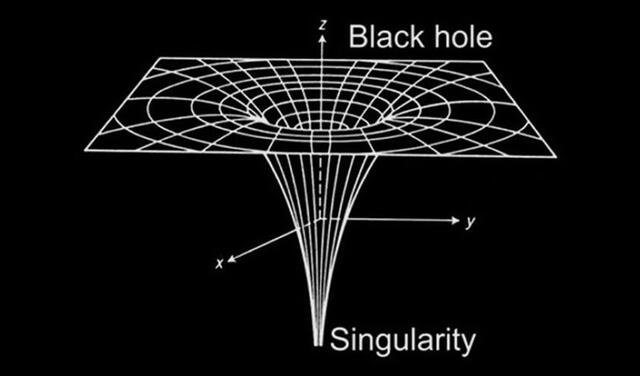
\includegraphics[scale=0.8]{negroagujero.jpeg}
      \end{center}
            
      \textbf{\large Geometric Interpretation}
      
      From the viewpoint of differential geometry, a \textbf{black hole} is a region of spacetime where curvature is so strong that it alters the causal structure. Timelike geodesics inside the horizon are all directed toward the singularity. This means that, once the horizon is crossed, the “future” of any particle inevitably leads to the center, which is not a choice but a geometric consequence.
      
      Thus, black holes are not “physical objects” in the classical sense, but regions defined by the \textbf{geometric structure} of spacetime, as determined by Einstein's equations.
      
      %%%%%%%%%%%%%%%%%%%%%%%%%%%%%%%%%%%%%%%%%%%%%%%%%%%%%%%%%%%%%%%%%%%%%%%%%%%

  \end{block}


  \begin{block}{Referencias}

    \nocite{*}
    \footnotesize{
      \bibliographystyle{plainnat}
      \bibliography{poster}
    }

  \end{block}

\end{column}
\separatorcolumn



\end{columns}
\end{frame}

\end{document}
